\documentclass[10pt]{scrartcl}
% \documentclass[10pt]{article}
\usepackage[T1]{fontenc}
\usepackage{amsmath,amsfonts,amssymb}
\usepackage{mathtools}
\usepackage{color,soul}
\usepackage{fullpage}
\usepackage{enumerate}
\usepackage{graphicx}
\usepackage[colorlinks=true,urlcolor=blue]{hyperref}
\usepackage{subcaption}
\usepackage{deluxetable}
\usepackage{verbatim}
\usepackage{fancyvrb}
\usepackage{listings}

\definecolor{Light}{gray}{.90}
\sethlcolor{Light}

\lstset{%
language=IDL,                   % choose the language of the code
basicstyle=\footnotesize\sffamily,%\ttfamily\footnotesize,       % the size of the fonts that are used for the code
numbers=left,                   % where to put the line-numbers
numberstyle=\footnotesize,      % the size of the fonts that are used for the line-numbers
stepnumber=1,                   % the step between two line-numbers. If it is 1 each line will be numbered
numbersep=5pt,                  % how far the line-numbers are from the code
showspaces=false,               % show spaces adding particular underscores
showstringspaces=false,         % underline spaces within strings
showtabs=false,                 % show tabs within strings adding particular underscores
% frame=single,                   % adds a frame around the code
backgroundcolor=\color{Light},
columns=flexible,
tabsize=2,                      % sets default tabsize to 2 spaces
captionpos=b,                   % sets the caption-position to bottom
breaklines=true,                % sets automatic line breaking
breakatwhitespace=false,        % sets if automatic breaks should only happen at whitespace
escapeinside={\%*}{*)}          % if you want to add a comment within your code
}

\title{Code Explanation}
\author{Jeren Suzuki}
\date{Last Edited \today}

\begin{document}

\maketitle
\pagenumbering{Roman}
\tableofcontents
\clearpage
\pagenumbering{arabic}

\section{Introduction} % (fold)
\label{sec:introduction}
This pdf is meant to illustrate what each step of the code is doing. The code is split up into four major parts. Preparing parameters, thresholding image to find suns, limb-fitting whole suns, and finding fiducials. 
% section introduction (end)

\section{Preparing Parameters} % (fold)
\label{sec:preparing_parameters}

\subsection{Loading Image} % (fold)
\label{sub:loading_image}
This is the starting image we use to analyze for sun centering and fiducial finding.
\begin{figure}[!ht]
    \centering
    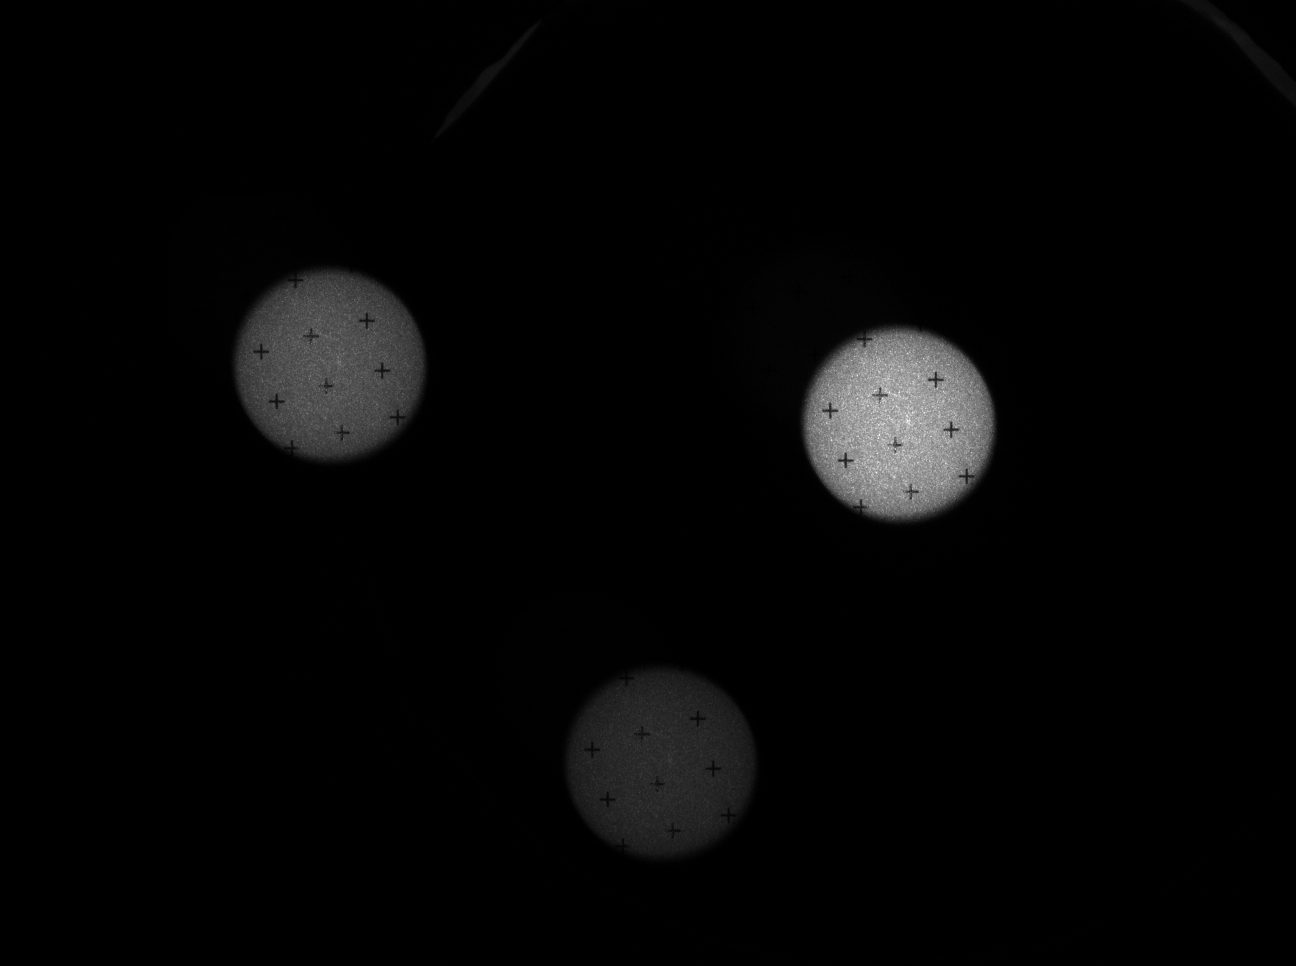
\includegraphics[width=.9\textwidth]{../plots_tables_images/tritest.jpg}    
    \caption{}
    \label{flowchart}
\end{figure}

% subsection loading_image (end)

\subsection{Reading In Parameter Block} % (fold)
\label{sub:reading_in_parameter_block}

\begin{lstlisting}
scan_width 10               ; Distance to next chord when picking chords to limb-fit
sundiam 70                  ; Approx Solar diameter, deprecated
nstrips 5                   ; Number of pairs of solar chords to limb-fit per direction
ministrip_length 4          ; Length of limb profile to linear fit
crop_box 120                ; Half-width of box used to find fiducials in
elim_perc 1                 ; Percentage of highest pixels to eliminate when finding threshold
n_smooth 900                ; Elements to smooth by when finding threshold 
border_pad 50               ; If solar center is within this value of border, marked as a partial sun
triangle_size .25           ; Percentage of image height to use for triangle sides for making clipped-bottom-corner mask
fid_smooth_thresh -150      ; Threshold to determine row/column positions of fiducials
onedsumthresh 80            ; Once looking at fiducial candidates, look at 1D sum of smaller fiducial crop and threshold difference of smoothed array - original array by this
disk_brightness 15          ; Arbitrary pixel brightness to eliminate bright fiducial candidates which are on the solar disk but are not on a fiducial
fid_crop_box 15             ; Half-width of box used to analyze fiducials
fid_smooth_candidates 15    ; Smoothing paramater for 1D sums of fiducial candidates 

\end{lstlisting}
% subsection reading_in_parameter_block (end)                 
% section preparing_parameters (end)

\section{Thresholding Image} % (fold)
\label{sec:thresholding_image}

After we read in the necessary parameters, we turn our attention to thresholding the image to find the centers of the suns. Starting with the initial image, we sort the image according to pixel values and see a grouping of differently dimmed suns. 

\begin{figure}[!ht]
    \centering
    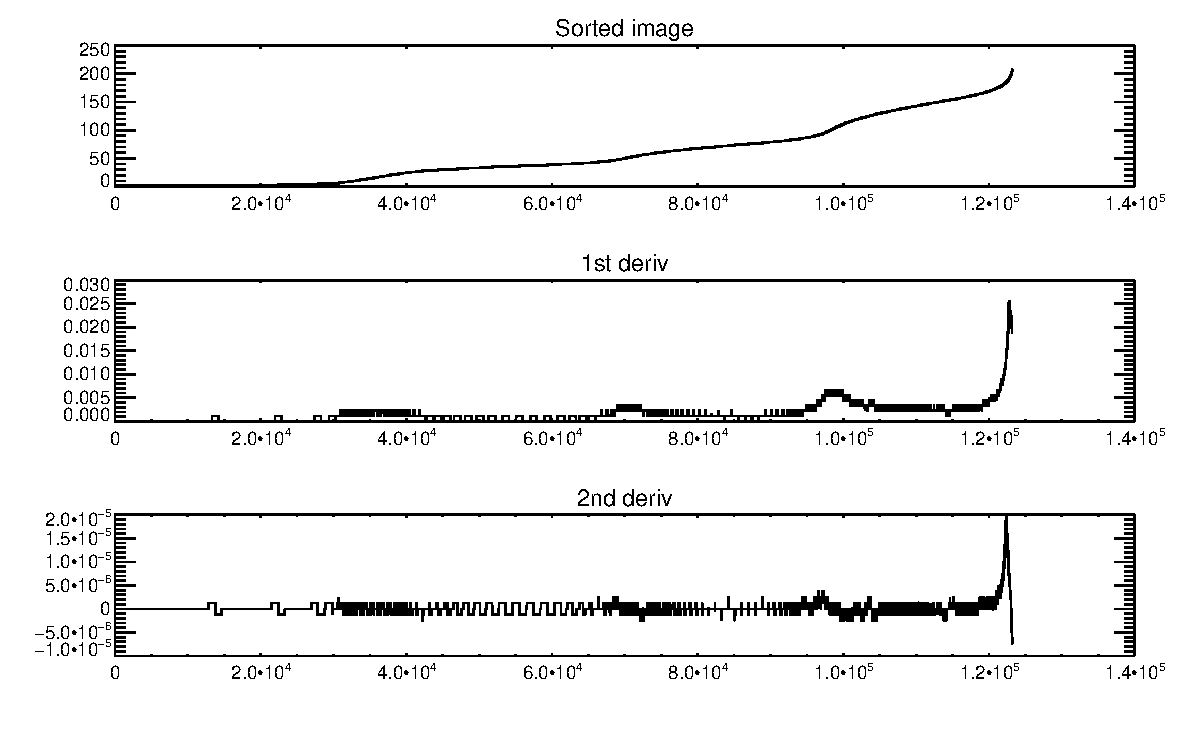
\includegraphics[width=.9\textwidth]{../plots_tables_images/sortedarray.eps}    
    \caption{We look at the second derivative because it consistently quantifies the thresholds to identify each solar region by. With the right-most part of the 2nd derivative zeroed out, we identify the three peaks corresponding to what pixel value we should threshold by to separately identify each sun.}
    \label{sortedarray}
\end{figure}

Using these three thresholds, we create separate masks, one for each sun. 

\begin{figure}[!ht]
    \begin{subfigure}[b]{.3\linewidth}
        \centering
        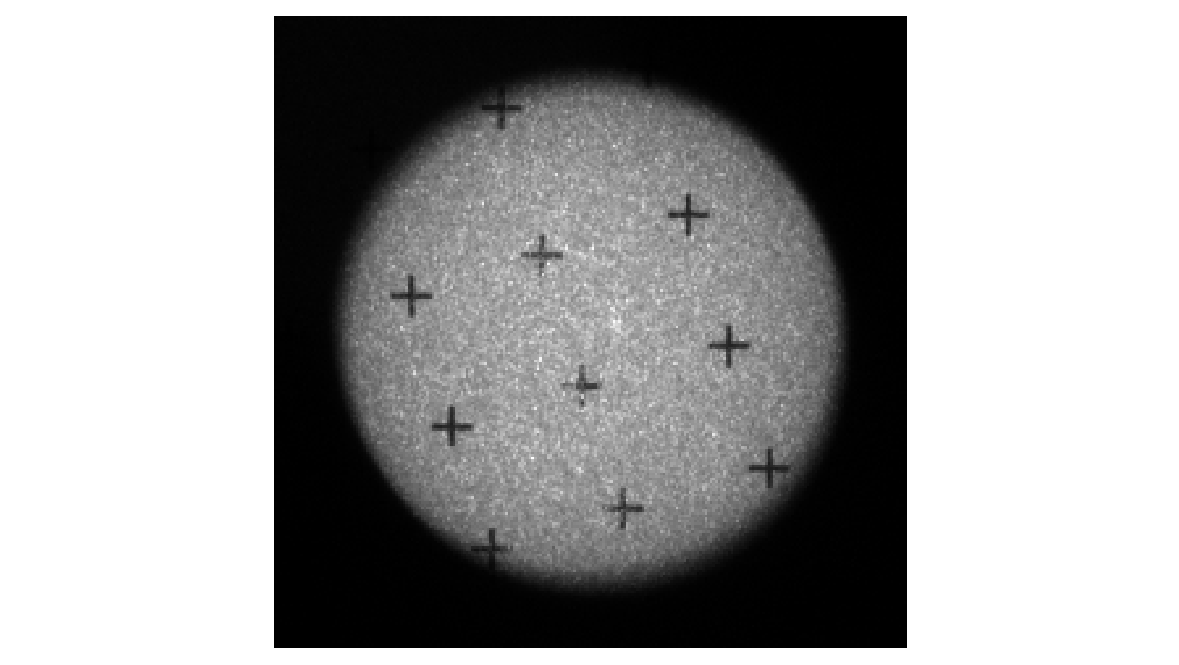
\includegraphics[width=1.3\textwidth]{../plots_tables_images/tritest_reg1}
        \caption{100\% brightness region, henceforth Region 1}
    \end{subfigure}
    \begin{subfigure}[b]{.3\linewidth}
        \centering
        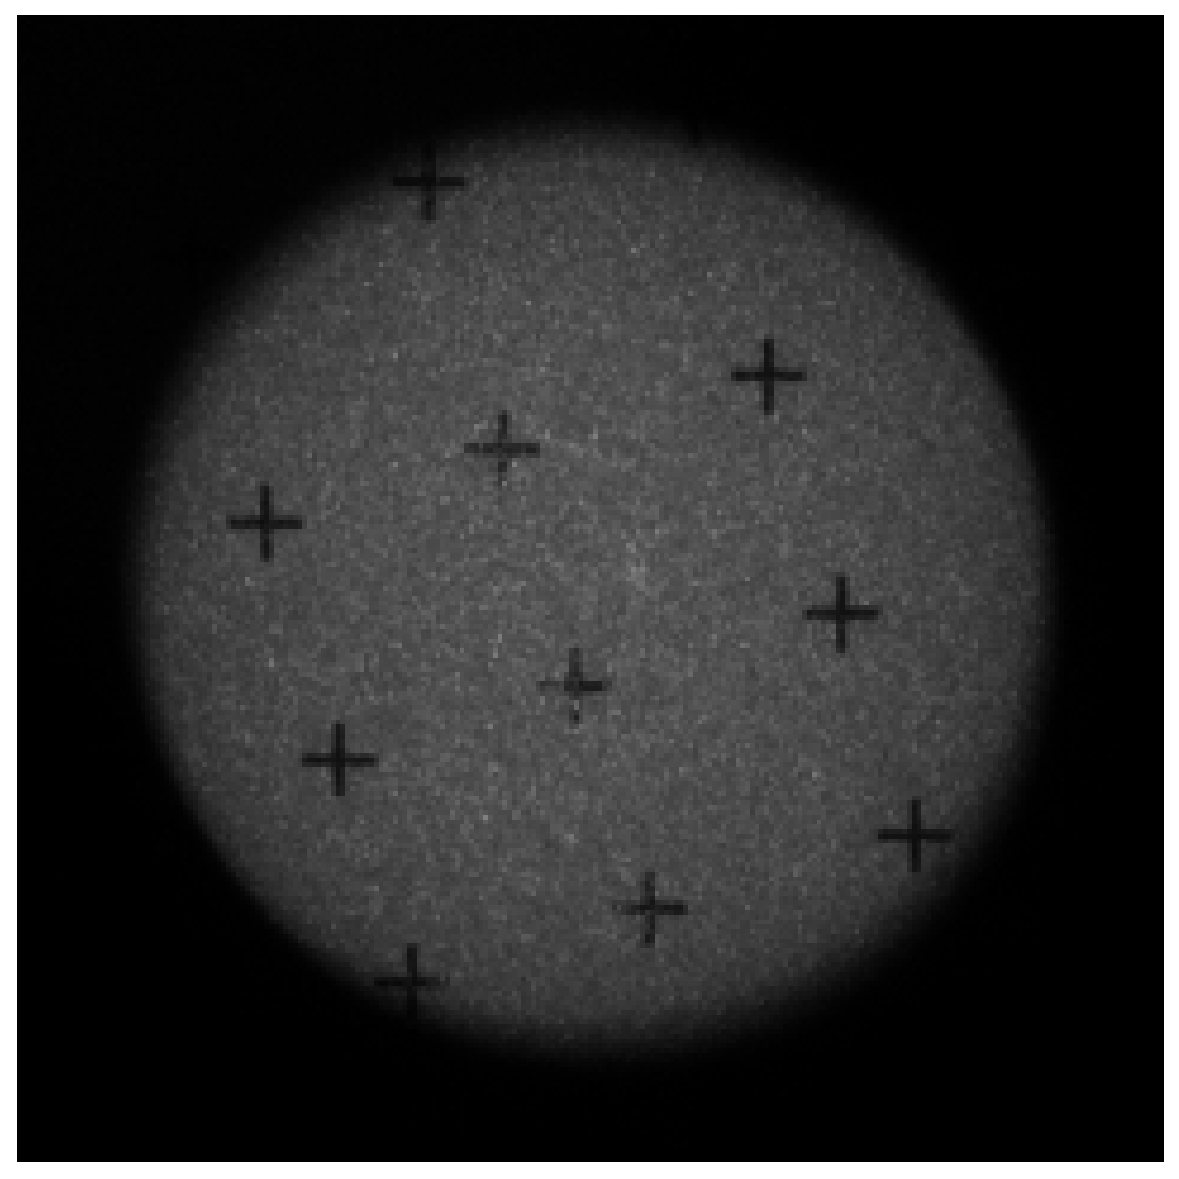
\includegraphics[width=1.3\textwidth]{../plots_tables_images/tritest_reg2}
        \caption{50\% brightness region, henceforth Region 2}
    \end{subfigure}
    \begin{subfigure}[b]{.3\linewidth}
        \centering
        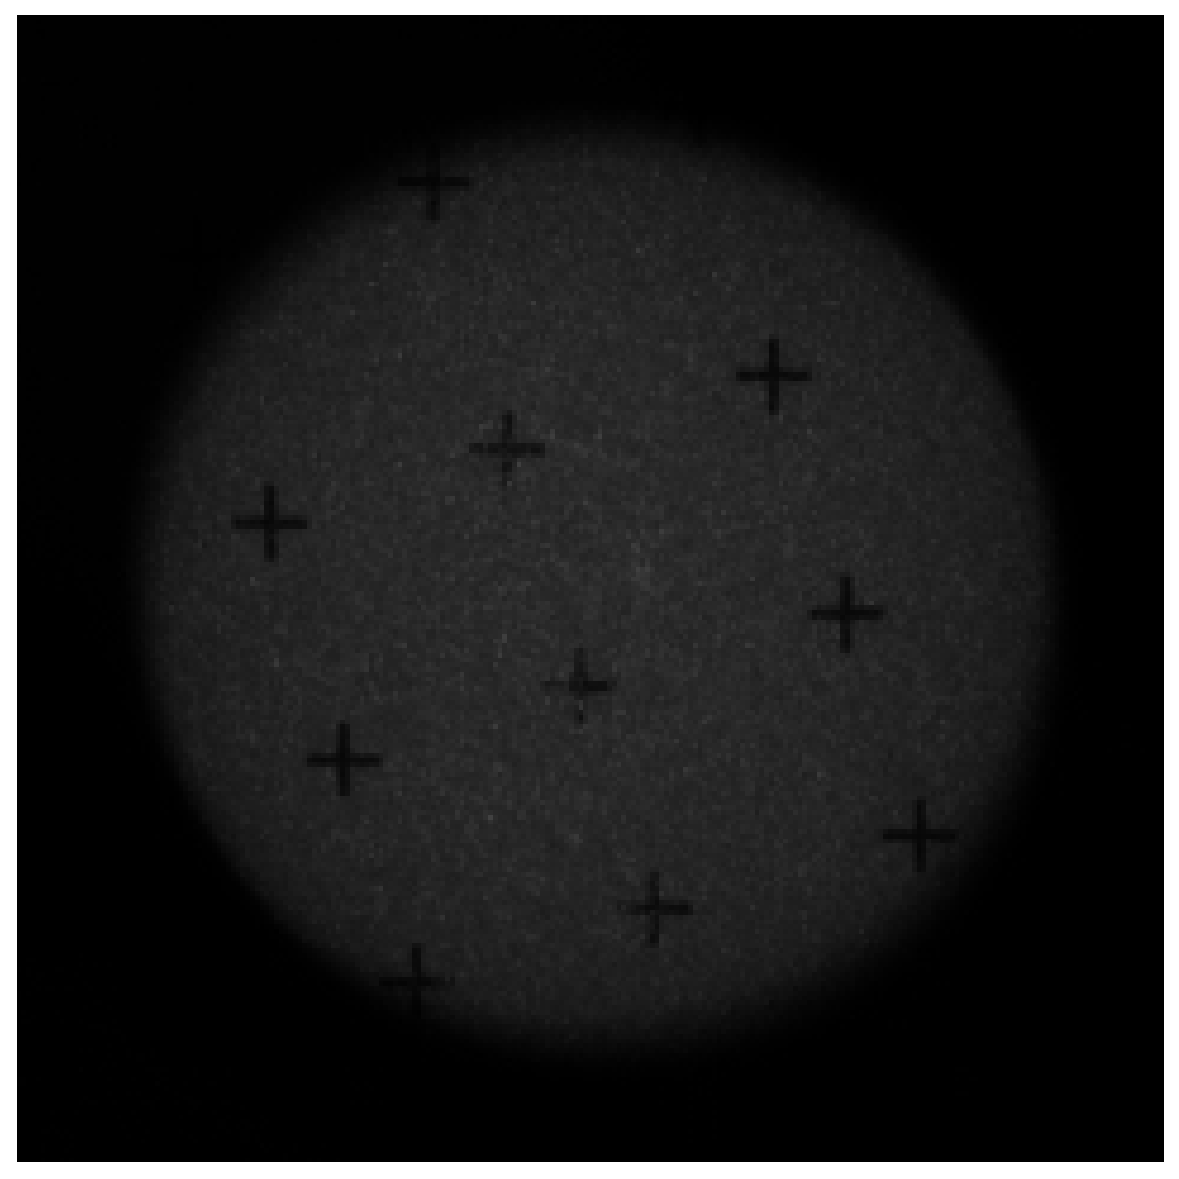
\includegraphics[width=1.3\textwidth]{../plots_tables_images/tritest_reg3}
        \caption{25\% brightness region, henceforth Region 3}
    \end{subfigure}
    \caption{}
    \label{triplecrop}
\end{figure}
% section thresholding_image (end)

\subsection{Quick mask centering} % (fold)
\label{sub:quick_mask_centering}

	Now that we have three cropped regions, we have to identify what brightnesses they are. We do this by looking at a low enough threshold that all the solar pixels for every brightness are included in the mask but not any of the background pixels. We then use IDL's \hl{\texttt{LABEL\_REGION}} to assign a label number to each shape. A shape is defined to be a mask where there are adjacent pixels. If done correctly, we end up with 3 shapes that have now had their values replaced with what index they have been assigned. For this image, we have three regions, one a mask of 1s, one a mask of 2s, and one of 3s. Now we use \hl{\texttt{HISTOGRAM}} to bin these shapes and thus their locations. For each mask, we calculate the average value of the pixels from the starting image and  






	We find the centers of each cropped region in Figure \ref{triplecrop} using a simple masking method. With the centroid determined by a simple masking method, we have to make sure that the center is from a whole sun. The process so far has not taken into account any spatial information so the next step is to look at a border region of the mask. 


\begin{figure}[!ht]
    \centering
    \hspace{-1.0in}
    \begin{subfigure}[b]{.45\linewidth}
        \centering
        
\includegraphics[width=1.3\textwidth]{../plots_tables_images/cutcorner.eps}
        \caption{What our mask should look like - side of black triangle is 1/4 of image width}
        \label{noborder}
    \end{subfigure}
    \hspace{.5in}
    \begin{subfigure}[b]{.45\linewidth}
        \centering
        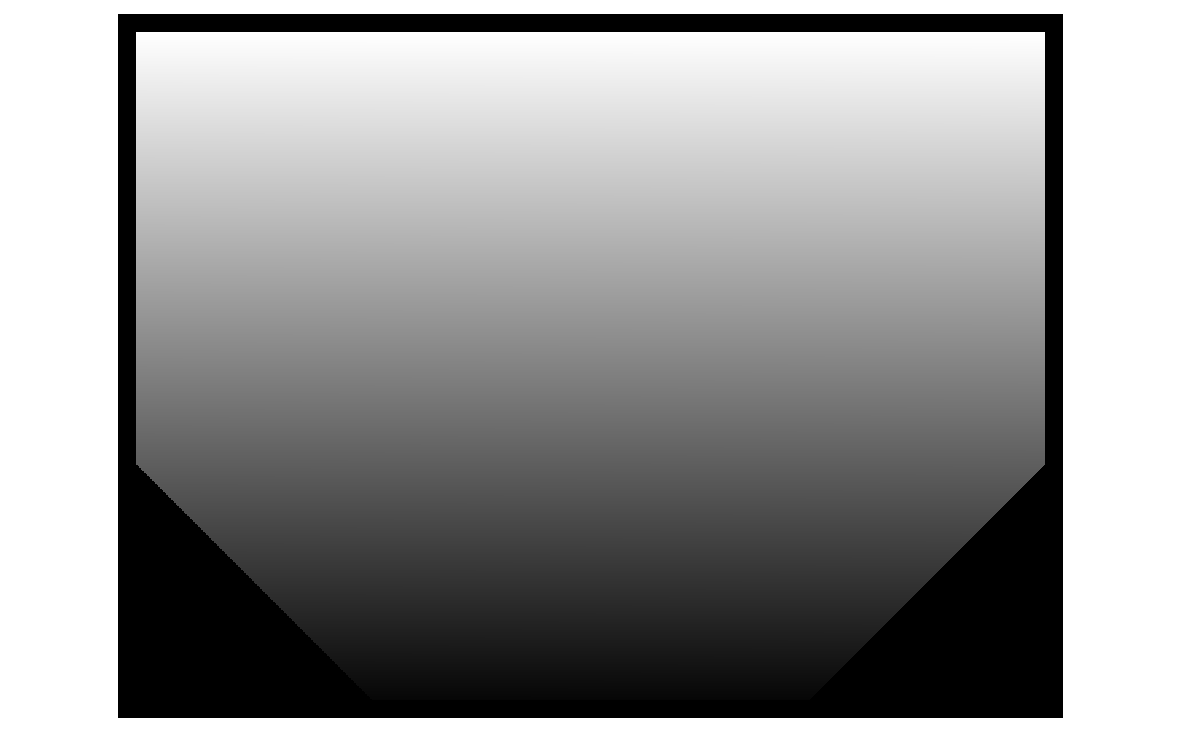
\includegraphics[width=1.3\textwidth]{../plots_tables_images/cutcornerwborder.eps}
        \caption{A proposed mask that looks within a certain distance form the border.}
        \label{aborder}
    \end{subfigure}
    \caption{The bottom corners will never see any data; the border mask takes into account the distance from the hypotenuse of the bottom corners}
    \label{cuttingcorners}
\end{figure}

If the center we computed with the mask method is within a certain distance to the edge of the image (as shown in Figure \ref{aborder}), we mark that solar region as ``\emph{partial}'' and cease further analysis for that particular brightness sun. \\
\indent Once we have our list of whole suns along with their masked centers, we proceed to fitting the solar limbs to find a more accurate center.
% subsection quick_mask_centering (end)

\section{Limb Fitting} % (fold)
\label{sec:limb_fitting}


% section limb_fitting (end)

\section{Finding Ficuials} % (fold)
\label{sec:finding_ficuials}

% section finding_ficuials (end)




\end{document}
